\begin{recipe}{Banana Bread}{\unit[1]{loaf}}{\unit[90]{minutes}}
\freeform This recipe is adapted from Baking Illustrated, an excellent, if anal-retentive cookbook from the editors of ``Cook's Illustrated'' magazine.
\newstep Preheat oven to \unit[350\0]{F.} Butter and flour a \unit[$5\times 9\times 3$]{inch} loaf pan.
\ing[2]{c.}{unbleached all-purpose flour}
\ing[1\fr12]{c.}{walnuts or pecans, chopped}
\ing[\fr34]{c.}{sugar}
\ing[\fr34]{tsp}{baking soda}
\ing[\fr12]{tsp}{salt}
Whisk together in a medium bowl.
\ing[3]{}{over-ripe bananas, mashed}
\ing[\fr13]{c.}{plain yogurt}
\ing[2]{}{eggs, lightly beaten}
\ing[6]{tbsp}{butter, melted and cooled}
\ing[1]{tsp}{vanilla extract}
Mix together with a rubber spatula. Lightly fold the banana mixture
into the dry ings until just combined. (Don't mix more than
necessary.) Scrape the batter into the loaf pan. Bake until a toothpick
inserted in the middle comes out clean, about one hour. Cool in the
pan for 5 or 10 minutes, then run a knife around the edges and turn
out onto a cutting board or cooling rack.
\end{recipe}
\begin{figure}[h!]
\begin{center}
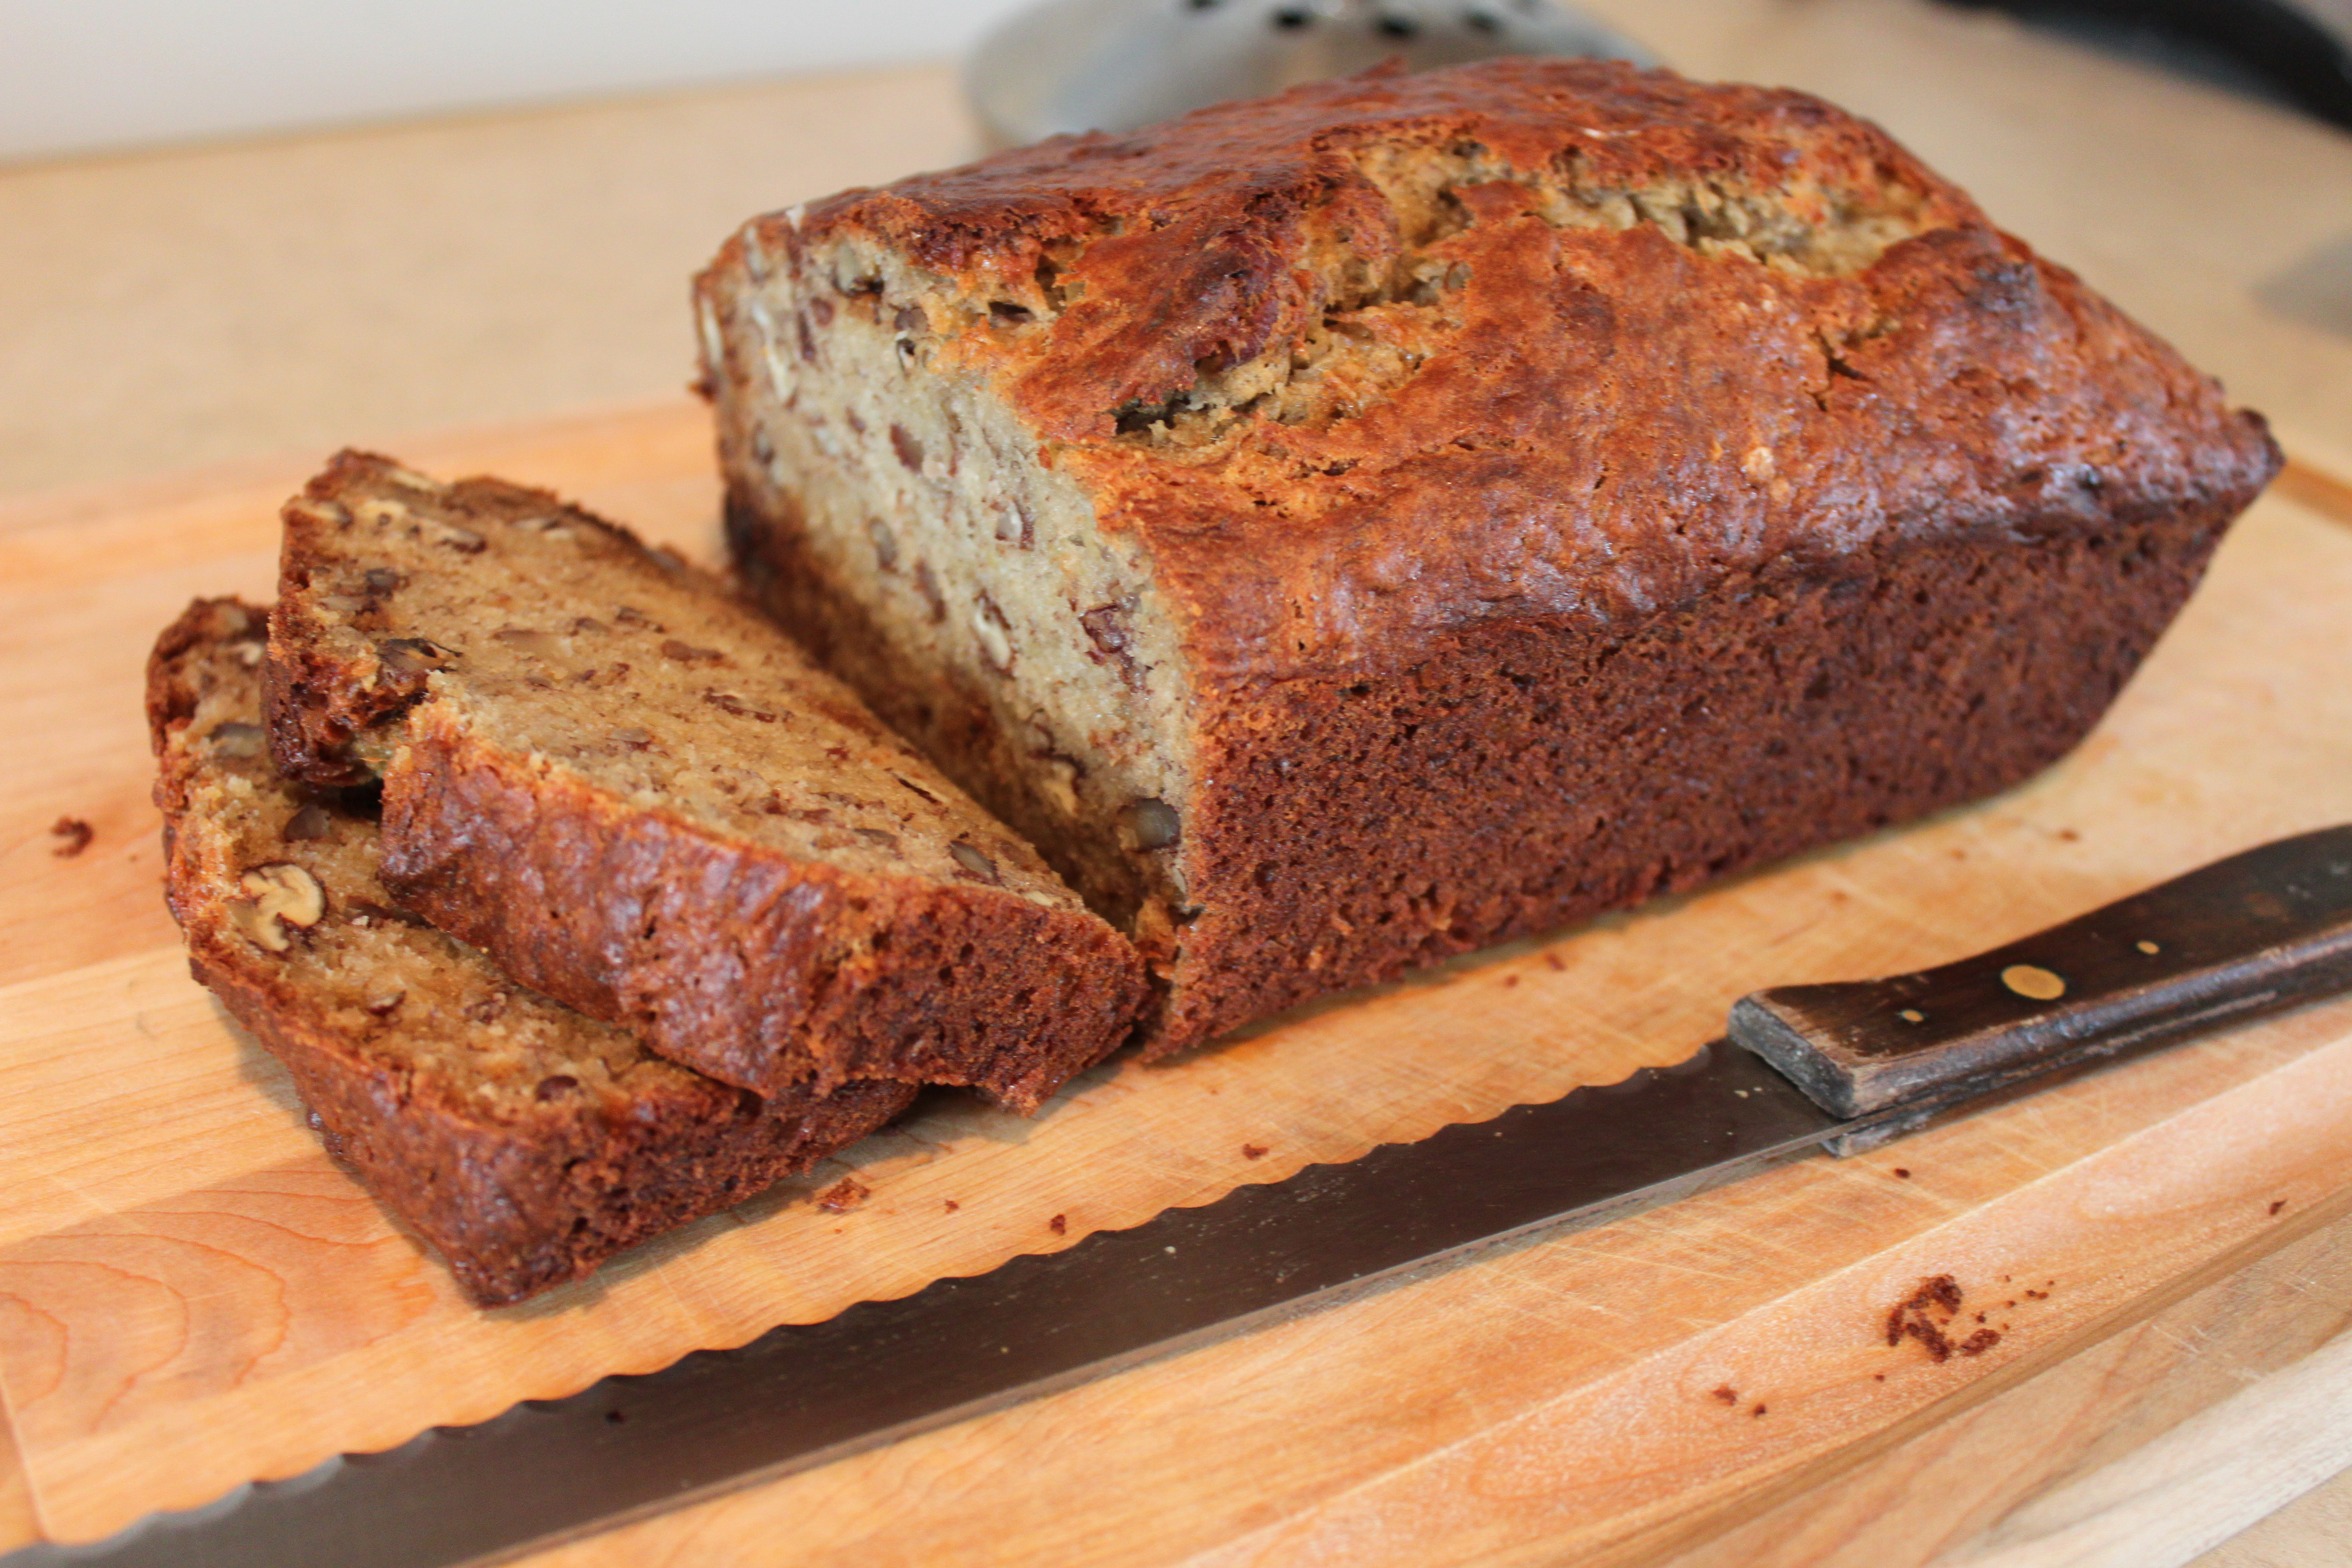
\includegraphics[height=0.26\textheight]{./figures/bananabread}
\end{center}
%\caption*{Yum.}
\end{figure}
